% This is samplepaper.tex, a sample chapter demonstrating the
% LLNCS macro package for Springer Computer Science proceedings;
% Version 2.20 of 2017/10/04
%
\documentclass[runningheads]{llncs}
%
\usepackage{graphicx}
\usepackage{hyperref}
% Used for displaying a sample figure. If possible, figure files should
% be included in EPS format.
%
% If you use the hyperref package, please uncomment the following line
% to display URLs in blue roman font according to Springer's eBook style:
% \renewcommand\UrlFont{\color{blue}\rmfamily}

\begin{document}
%
\title{Chess Num - PLOG 2020}
%
%\titlerunning{Abbreviated paper title}
% If the paper title is too long for the running head, you can set
% an abbreviated paper title here
%
%\author{João Lucas Silva Martins - 201806436 \and João de Jesus Costa - 201806560}
\author{FEUP-PLOG, Turma 3MIEIC03, Grupo 3}

\institute{Faculty of the engeenirings of the universities of feup}
\maketitle

\begin{abstract}
This paper is a brief analysis of our solution of the 
\href{https://erich-friedman.github.io/puzzle/chessnum/}{Chess-Num} problem, developed
in the context of the PLOG U.C. The solution is implemented using sicstus prolog and its
clpfd constraints library. TODO copiar conclusao para aqui

%\keywords{First keyword  \and Second keyword \and Another keyword.}
\end{abstract}
%
%
%
\section{Template}
\subsection{A Subsection Sample}
Please note that the first paragraph of a section or subsection is
not indented. The first paragraph that follows a table, figure,
equation etc. does not need an indent, either.

Subsequent paragraphs, however, are indented.

\subsubsection{Sample Heading (Third Level)} Only two levels of
headings should be numbered. Lower level headings remain unnumbered;
they are formatted as run-in headings.

\paragraph{Sample Heading (Fourth Level)}
The contribution should contain no more than four levels of
headings. Table~\ref{tab1} gives a summary of all heading levels.

\begin{table}
\caption{Table captions should be placed above the
tables.}\label{tab1}
\begin{tabular}{|l|l|l|}
\hline
Heading level &  Example & Font size and style\\
\hline
Title (centered) &  {\Large\bfseries Lecture Notes} & 14 point, bold\\
1st-level heading &  {\large\bfseries 1 Introduction} & 12 point, bold\\
2nd-level heading & {\bfseries 2.1 Printing Area} & 10 point, bold\\
3rd-level heading & {\bfseries Run-in Heading in Bold.} Text follows & 10 point, bold\\
4th-level heading & {\itshape Lowest Level Heading.} Text follows & 10 point, italic\\
\hline
\end{tabular}
\end{table}


\noindent Displayed equations are centered and set on a separate
line.
\begin{equation}
x + y = z
\end{equation}
Please try to avoid rasterized images for line-art diagrams and
schemas. Whenever possible, use vector graphics instead (see
Fig.~\ref{fig1}).

\begin{figure}
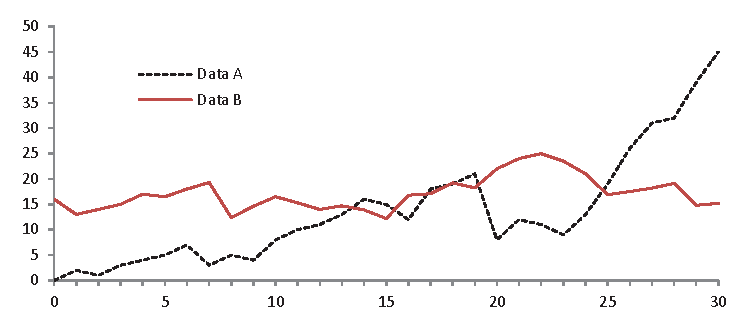
\includegraphics[width=\textwidth]{fig1.eps}
\caption{A figure caption is always placed below the illustration.
Please note that short captions are centered, while long ones are
justified by the macro package automatically.} \label{fig1}
\end{figure}

\begin{theorem}
This is a sample theorem. The run-in heading is set in bold, while
the following text appears in italics. Definitions, lemmas,
propositions, and corollaries are styled the same way.
\end{theorem}
%
% the environments 'definition', 'lemma', 'proposition', 'corollary',
% 'remark', and 'example' are defined in the LLNCS documentclass as well.
%
\begin{proof}
Proofs, examples, and remarks have the initial word in italics,
while the following text appears in normal font.
\end{proof}
For citations of references, we prefer the use of square brackets
and consecutive numbers. Citations using labels or the author/year
convention are also acceptable. The following bibliography provides
a sample reference list with entries for journal
articles~\cite{ref_article1}, an LNCS chapter~\cite{ref_lncs1}, a
book~\cite{ref_book1}, proceedings without editors~\cite{ref_proc1},
and a homepage~\cite{ref_url1}. Multiple citations are grouped
\cite{ref_article1,ref_lncs1,ref_book1},
\cite{ref_article1,ref_book1,ref_proc1,ref_url1}.

\section{Introduction}


In this paper we describe our solution to the \href{https://erich-friedman.github.io/puzzle/chessnum/}{Chess-Num}
problem, which can solve any instance of the puzzle, generate a random solution,
while presenting the result in a human readable way.
We first begin by describing the problem, afterwards we explain our prolog approach,
then we analyse the solution's complexity.

Even tough we tried to find other approaches/references to the problem, we couldn't find any.

\section{Problem Description}

The Chess-Num problem is a chess puzzle in which, given a set of
numbered cells in the chess board, one tries to place six chess pieces
(rook, queen, king, bishop, knight pawn) in a way that the number of each
given cell corresponds to the number of attacking pieces of that cell.
See this \href{https://erich-friedman.github.io/puzzle/chessnum/}{link} for further description and
examples.

\section{Approach}
\subsection{Decision Variables}

The decision variables correspond to the pair coordinates for each piece. They all
are within the domain [0, 7] . Also, all pairs are distinct between each other and the given
numbered cells' coordinates.

\subsection{Constraints}
\section{Solution Presentation}
\section{Experiments and Results}
\section{Conclusions and Future Work}

\section{References}
\section{Annex}
\end{document}
